\chapter{Subespaços Vetoriais}
\thispagestyle{empty}

\section{Introdução}
Um espaço vetorial pode ser um conjunto muito grande e às vezes  pode ser útil identificar outros espaços vetoriais dentro dele. Espaços vetoriais que estão dentro de outros espaços vetoriais são chamados de subespaços vetoriais.   \textbf{Atenção.} \textit{Estas notas de aulas tem como objetivo guiar os alunos nos  estudos da disciplina álgebra linear, nas turmas de minha responsabilidade, nos cursos de engenharia da UNIVASF. O uso das mesmas  não dispensa  a leitura  dos livros didáticos indicados nas referências bibliográficas da disciplina, bem como a resolução de exercícios propostos nos mesmos}.

\section{Subespaço Vetorial}


\textbf{Definição.} Sejam $V$ um espaço vetorial e $ W$ um subconjunto  não vazio de $V$.  O subconjunto  $W$ é um \textbf{subespaço vetorial} de $V$,  se $W$ é um espaço vetorial  em relação as operações  de adição de vetores e multiplicação por escalar definidas em $V$.

\vspace{0.3cm}

De acordo com a definição anterior, qualquer subespaço de  um espaço vetorial  $V$ deve, necessariamente, conter o vetor nulo de $V$. De fato, a operação de adição de vetores a ser considerada no subconjunto $W$ é  obrigatoriamente a mesma de $V$ e o elemento neutro dessa operação é único.  A Figura \ref{fig:subespaco} ilustra esse fato.



\begin{figure}[h!]
\center
% \includegraphics[width=0.7\textwidth]{subespaco}
\caption{\footnotesize{Um subespaço vetorial é um espaço vetorial dentro de outro}}
\label{fig:subespaco}
\end{figure}


%\vspace{0.3cm}
Todo espaço vetorial $V$ admite pelo menos dois subespaços: o conjunto formado apenas pelo vetor nulo  e o próprio espaço. Isto é,  $\{ 0\}$ e  $V$. Esses dois subespaços de $V$  são chamados de \textbf{subespaços triviais}.

%\vspace{0.3cm}

Utilizar a definição de subespaço vetorial para  identificar se um subconjunto $W$  de um espaço vetorial $V$  é um subespaço é  uma atividade laboriosa, pois exige a verificação das oito propriedades,  (A1)-(A4) e (ME1)-(ME4), da definição de espaço vetorial. Felizmente, de acordo com a  próxima proposição,  não precisaremos fazer  a verificação de todas essas propriedades. De fato, sendo  $W$  um subconjunto de $V$,  as propriedades  das operações que são válidas em $V$ devem também ser válidas em $W$, desde que $W$ seja um conjunto fechado em relação a essas operações. Isto é, o resultado das operações realizadas com elementos de $W$  resultam em elementos de $W$.

 Um subespaço vetorial $W$ de um espaço vetorial $V$  fica caracterizado pela seguinte proposição:

\textbf{Proposição.} Dados um espaço vetorial $V$ e  um subconjunto $W$ de $V$   não vazio. $W$ é um subespaço de  $V$ se as duas condições a seguir  forem satisfeitas:

\begin{enumerate}[label=(\roman*)]
\item Se $u$ e $v$ são vetores quaisquer de $W$, então $u+v \in W$;
\item Se  $ \alpha \in \mathbb{R}$ e $ v$ é um vetor qualquer de $W$, então $\alpha v\in W$.

\end{enumerate}

\textbf{\textit{Observações.}}
\begin{enumerate}%[label=(\roman*)]
\item Todo subespaço $W$ de um espaço vetorial $V$ precisa, necessariamente, conter o vetor nulo de $V$. De fato, se tomarmos $\alpha=0$, por (ii),  temos $$0\cdot v=0 $$ para todo $v \in W$.

\item Dessa forma,  se um subconjunto não vazio  $W$ de um espaço vetorial $V$ não possuir o vetor nulo de $V$,  então $W$ não pode ser um subespaço vetorial de $V$.
\end{enumerate}

\section{Exemplos}
\begin{enumerate}


\item Seja $V=\mathbb{R}^2=\{(x_1, x_2); x_i \in \mathbb{R}\}$ com as operações usuais de  soma de vetores e a multiplicação por escalar.  O subconjunto
$$W=\{(x, y); y=kx, \; \text{$k$ é uma constante} \}$$ é um subespaço vetorial de $V$.

\textbf{\textit{Demonstração.}}
Observe que $W$ também pode ser escrito da seguinte maneira:
$$W=\{(x, kx);  x \in \mathbb{R} \; \text{e}\; \text{$k$ constante} \}.$$   Primeiro é conveniente observar que $(0,0) \in W$. De fato, para $x=0$ teremos $kx=0$, para todo $k\in \mathbb{R}$. Logo, $(0,0) \in W$ e, desse modo, $W \neq \emptyset$.

Agora sejam $u=(x_1, y_1)$ e $v=(x_2, y_2)$ vetores de $W$.  Dessa maneira, podemos escrever $u=(x_1, kx_1)$ e $v=(x_2, kx_2)$. Assim,
\begin{align*}
u+v &=(x_1, kx_1)+(x_2, kx_2)\\
       &=(x_1+x_2, kx_1+kx_2)\\
       &=(x_1+x_2, k(x_1+x_2)).
\end{align*}
Fazendo $x_3=x_1+x_2$, temos que $u+v =(x_3, kx_3)$. Logo, $u+v \in W$ e o item (i) é satisfeito.  Agora seja  $\alpha \in \mathbb{R}$ e $u=(x_1, y_1) \in W$. Assim
\begin{align*}
\alpha u &=\alpha(x_1,x_2)\\
            &=\alpha (x_1, kx_1) \; \text{pois} \;  u \in W;\\
       &=(\alpha x_1, \alpha k x_1).
\end{align*}
 Fazendo $x_4=\alpha x_1$ temos que $\alpha u=(x_4, kx_4)$. Logo, $\alpha u \in W$ e o intem (ii) da proposição está satisfeito.  Poranto, $W$ é um subespaço vetorial de $V$. Observe ainda que os elementos de  $W$ descrevem uma reta passando pela origem.

\item Seja $V=\mathbb{R}^2$ e $U=\{(x, 5x+3);  x \in \mathbb{R}\}$.  O subconjunto $U$,  com as operações usuais de  soma de vetores e a multiplicação por escalar,não é um subespaço vetorial de $\mathbb{R}^2$.   De fato,  o vetor $\{(0,0\}$ não pertence a $W$. Observe que os elementos de $U$ descrevem uma reta em $\mathbb{R}^2$ que não passa pela origem.


\item Todos os subespaços de $\mathbb{R}^2$ são:  $\{(0,0)\}$, o  $\mathbb{R}^2$  e os seus subconjuntos que descrevem  retas passando pela origem.

\item Seja $W=\{(x,y,z) \in \mathbb{R}^3; ax+by+cz=0\}$.  Observe que $W$ descreve, em $\mathbb{R}^3$, um \textbf{plano que passa pela origem}.  $W$ é um subespaço vetorial de $\mathbb{R}^3$.

\textbf{\textit{Demonstração.}}
  Primeiro é conveniente observar que $(0,0,0) \in W$. De fato, para $x=y=z=0$ teremos $ax+by+cz=0$, quaisquer que sejam os escalares  $a,b,c \in \mathbb{R}$. Logo, $(0,0,0) \in W$ e, desse modo, $W \neq \emptyset$.

Agora sejam $u=(x_1, y_1, z_1)$ e $v=(x_2, y_2, z_2)$ vetores de $W$.  Dessa maneira,  temos que $ax_1+bx_1+cz_1=0$ e  $ax_2+bx_2+c_z2=0$. Assim,  temos
\begin{align*}
u+v &=(x_1, y_1, z_1)+(x_2, y_2, z_2)\\
       &=(x_1+x_2, y_1+y_2, z_1+z_2).
\end{align*}
Fazendo $x_3=x_1+x_2$,$y_3=y_1+y_2$ e $z_3=z_1+z_2$ temos que
\begin{align*}
ax_3+by_3+cz_3&=a(x_1+x_2)+b(y_1+y_2)+c(z_1+z_2)\\
                             &=\underbrace{ax_1+by_1+cz_1}_{0}+\underbrace{ax_2+by_2+cz_2}_{0}\\
                             &=0+0=0.
\end{align*}
Logo, $u+v  \in W$ e o item (i) é satisfeito.  Agora seja  $\alpha \in \mathbb{R}$ e $u=(x_1, y_1, z_1) \in W$. Assim, $ax_1+bx_1+cz_1=0$.
\begin{align*}
\alpha u &=\alpha(x_1,y_1, z_1)\\
            &=\alpha (x_1,y_1, z_1) \\
       &=(\alpha x_1, \alpha y_1, \alpha z_1).
\end{align*}
 Fazendo $x_4=\alpha x_1$, $y_4=\alpha y_1$ e  $z_4=\alpha z_1$ temos que
\begin{align*}
ax_4+by_4+cz_4&=a(\alpha x_1)+b(\alpha y_1)+c(\alpha z_1)\\
                              &=\alpha ( ax_1 +b y_1+cz_1)\\
                             &=\alpha\underbrace{ax_1+by_1+cz_1}_{0}\\
                             &=\alpha \cdot 0=0.
\end{align*}
Logo, $\alpha u \in W$ e o intem (ii) da proposição está satisfeito.  Portanto, $W$ é um subespaço vetorial de $\mathbb{R}^3$.


\item Todos os subespaços de $\mathbb{R}^3$ são:  $\{(0,0,0)\}$, o  $\mathbb{R}^3$, os seus subconjuntos que descrevem  retas passando pela origem e os subconjuntos que descrevem planos passando pela origem.


\item Considere em $\mathbb{M}(n,n)$  o conjunto $S$ das matrizes simétricas de ordem $n$.  $S$ é um subespaço vetorial de $\mathbb{M}(n,n)$ . Isto é, $$S=\{ A \in \mathbb{M}(n,n); A^T=A\}.$$ $S$ é um subespaço vetorial de $\mathbb{M}(n,n)$ .

\textbf{\textit{Demonstração.}}
Primeiro observe que a matriz nula de ordem $n$ é uma matriz simétrica. Logo, $ S \neq \emptyset$.  Agora sejam $A$ e $B$ matrizes simétricas de ordem $n$. Pela propriedade das matrizes  simétricas, temos que $$ (A+B)^T=A^T+B^T. $$
Por outro lado, $A$ e $B$ são matrizes simétricas. Logo, $A^T=A$ e $B^T=B$. Daí, vem que  $$ (A+B)^T=A^T+B^T = A +B .$$ Ou seja, $A+B$ é uma matriz simétrica. Logo, $A+B \in  \mathbb{M}(n,n)$.

Dado $\alpha \in \mathbb{R}$ e $A$ uma matriz simétrica de ordem $n$, temos, pela propriedade de matriz simétrica, que  $$(\alpha A)^T= \alpha A^T=\alpha A.$$ Assim, $\alpha A$ é uma matriz simétrica, ou seja, $\alpha A \in \mathbb{M}(n,n)$. Portanto, $S$ é um subespaço vetorial de $\mathbb{M}(n,n)$.


\item Considere o sistema linear homogêneo $$AX=0$$ onde  $A$, a matriz dos coeficientes, tem  ordem $m \times n$, $X$ é a matriz das incógnitas  e tem ordem $n \times 1$ e $0$ pé matriz dos termos independentes e tem ordem $ m \times 1$.  Seja $S_h$ o conjunto das soluções desse sistema linear homogêo.  Isto é,
$$S_h=\{ X \in \mathbb{M}(n,1); AX=0 \}.$$  $S_h$ é um subespaço vetorial de $\mathbb{M}(n,n)$ .
\end{enumerate}

\subsection{Intersecção de Subespaços}
Seja  $V$ um espaço vetorial sobre um corpo $\mathbb{K}$. Suponha que $U$ e $W$ são  subespaços vetoriais de $V$. Então o conjunto
$$U\cap W=\{ v \in V;  \; v \in U \; \text{e} \; v \in W \} $$ é um subespaço vetorial de $V$.

\textbf{\textit{Demonstração.}}

Primeiro note que $U\cap W \neq \emptyset$. Isto é, $0 \in U\cap W$. De fato,  como $U$ e $W$ são subespaços de $V$, então $0 \in U$ e $0 \in W$, logo $0 \in U\cap W$.

Agora, vamos mostrar que a soma de dois vetores quaisquer de $U \cap W$ é um vetor de  $U \cap W$.  Para isso suponha que $u,v \in U\cap W$. Dessa forma temos:
\begin{align*}
u\in U\cap W&, \; \text{ logo $u \in U$ e $u \in W$};\\
v\in U\cap W &, \; \text{logo  $v \in U$ e $v \in W$}.
\end{align*}
Dessa maneira, temos  $u, v \in U$;   e $u,v \in W$. Como $U$ e $W$ são subespaços, então $u+ v \in U$  e $u+v \in W$. Logo, $$u+ v \in U \cap W. $$

Para mostrarmos que a multiplicação de um vetor de $U\cap W$ por um escalar  também é um vetor $U\cap W$,  considere $\alpha \in \mathbb{K}$  e $u \in U\cap W$.  Desse modo,  $u\in U$ e $u \in W$  (ambos são subespaços de $V$), então   $\alpha \cdot  u \in U$ e $\alpha \cdot  u \in W$.
Logo, $\alpha \cdot  u\in U\cap W$. Dessa forma concluimos que $U\cap W$ é um subespaço vetorial de $V$.

\subsubsection{\textbf{Exemplos}}
\begin{enumerate}
\item Considere os subespaços de $\mathbb{R}^3$
$$ U= \{(x,y,z) \in \mathbb{R}^3 ; z=0\} $$ e  $$ W= \{(x,y,z) \in \mathbb{R}^3 ; x=0\}.  $$ Seja $(a, b, c)$ um vetor qualquer de $\mathbb{R}^3$. Observe que  $(a, b,c ) \in U\cap W$ se, e somente se,  $(a, b, c) \in U$ e $(a, b, c) \in W$, simultaneamente. Mas, isso somente ocorre se tivermos  $a=0$   e $c=0$. Logo, um  vetor $v$ do $\mathbb{R}^3$ está em $U \cap W$ se, e somente se, $v$ é do tipo $(0, b, 0)$. Assim, escrevemos $$U \cap W=\{(x, y, z) \in\mathbb{R}^3; x=z=0 \}=\{ (0,y,0); y \in \mathbb{R}\}.$$


\item Considere em $\mathbb{R}^2$ os subespaços
$$ U= \{(x,y) \in \mathbb{R}^2 ; y=x\} $$ e  $$ W= \{(x,y) \in \mathbb{R}^2 ; y=-x\}.  $$ Seja $(a, b)$ um vetor qualquer de $\mathbb{R}^2$. Observe que  $(a, b ) \in U\cap W$ se, e somente se,  $(a, b) \in U$ e $(a, b) \in W$, simultaneamente. Mas, isso ocorre somente  se tivermos  $b=a$   e $b=-a$. De onde concluímos que $b=0$ e $a=0$.  Logo, um  vetor $v$ do $\mathbb{R}^2$ está em $U \cap W$ se, e somente se, $v=(0, 0)$. Assim, obtemos $$U \cap W=\{(0,0) \}.$$

\item  Sejam $V= \mathbb{M}(n,n)$ seja o espaço vetorial  das matrizes quadradas, com entradas reais,  de ordem $n$; $U$ o subconjunto  das matrizes triangulares inferiores e $W$ o subconjunto das matrizes triangulares superiores de ordem $n$.  É possível mostrar que $U$ e $W$ são subespaços vetoriais de $V$ (Exercício).  Observe que $U \cap W$ é o conjunto de todas as matrizes diagonais de ordem $n$.
\end{enumerate}

Sobre a reunião, $U \cup W$, de dois subespaços $U$ e $W$ de um dado espaço vetorial $V$ podemos dizer que, em geral, não é um subespaço vetorial de $V$. A Figura \ref{fig:intersect} ilustra a união e a intersecção de subconjuntos de $V$.

\begin{figure}[h!]
	\center
	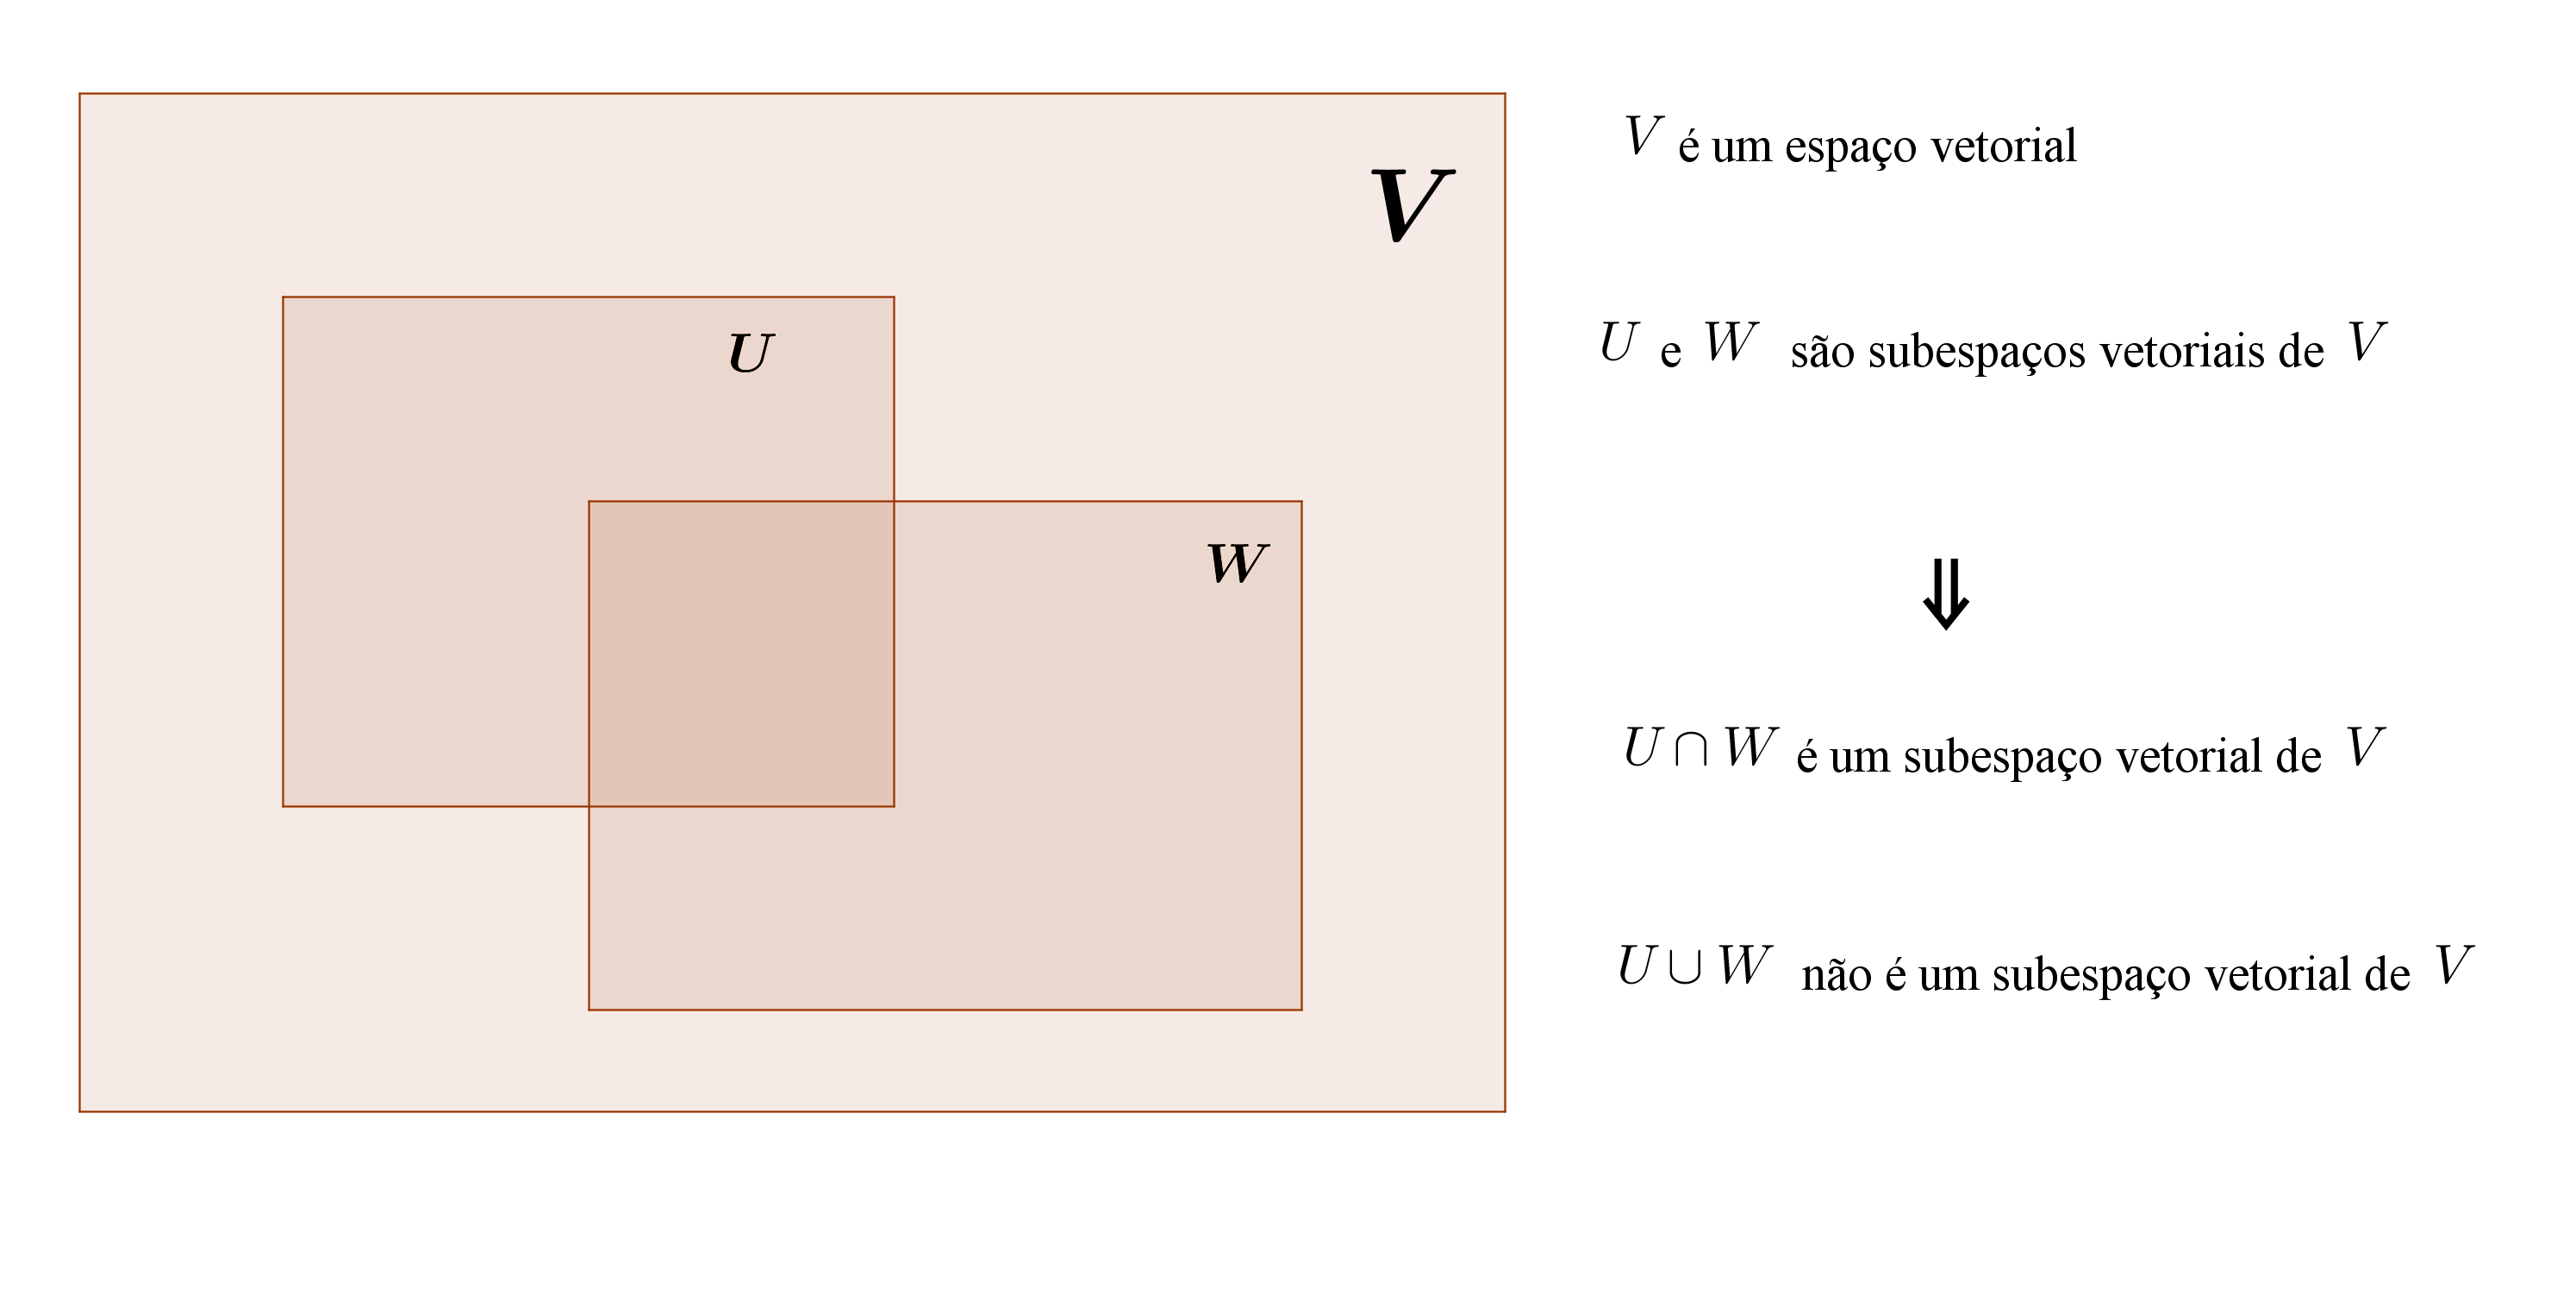
\includegraphics[width=0.7\textwidth]{chapters/subespacos_vetoriais/img/intersect}
	\caption{\footnotesize{A intersecção de subespaços vetoriais é um subespaço vetorial}}
	\label{fig:intersect}
\end{figure}

Mostraremos que a reunião de dois subespaços nem sempre é um subespaço vetorial, apresentando um exemplo no espaço vetorial $\mathbb{R}^2$. Considere os seguintes subespaços vetoriais de $\mathbb{R}^2$:  $$U=\{(x, 0); x \in \mathbb{R}\} \;\;\text{e} \;\;  W=\{(0, y); y \in \mathbb{R} \}.$$ Observe que o vetor $(2,0) \in U$  e o vetor $(0,5) \in W$. Logo, ambos pertencem ao conjunto  $U \cup W$. No entanto, a soma desses dois vetores $$(2,0)+(0,5)=(2,5)$$ não é um vetor de $U$ nem um vetor $W$. Logo, não é um vetor de $U \cup W$. Portanto, $U \cup W$ não é um subespaço vetorial de $\mathbb{R}^2$.







\subsection{Soma de Subespaços}
Seja  $V$ um espaço vetorial sobre um corpo $\mathbb{K}$. Suponha que $U$ e $W$ são  subespaços vetoriais de $V$. Então o conjunto
$$U+W=\{ v \in V; v=v_1+v_2, \; v_1 \in U \; \text{e} \; v_2 \in W \} $$ é um subespaço vetorial de $V$. O subespaço $U+W$ chama-se \textit{ soma} de $U$ e $W$.

\textbf{\textit{Demonstração.}}

Primeiro note que $U+W \neq \emptyset$. Isto é, $0 \in U+W$. De fato,  como $U$ e $W$ são subespaços de $V$, $0 \in U$ e $0 \in W$. Desse modo, como  $$0=0+0,$$ temos que $0$ pode ser escrito como a soma de um elemento de $U$ com um elemento de $W$.

Sejam $u,v \in U+W$. Dessa forma podemos escrever
\begin{align*}
u&=u_1+w_1, \; \text{com $u_1 \in U$ e $w_1 \in W$};\\
v&=u_2+w_2, \; \text{com $u_2\in U$ e $w_2 \in W$}.
\end{align*}
Assim, como $u_1, u_2 \in U$ (e $U$ é um subespaço de $V$), então $u_1+u_2 \in U$.  Do mesmo modo, como $w_1, w_2 \in W$ (e $W$ é um subespaço de $V$), então $w_1+w_2 \in W$.

Desse modo,
\begin{align*}
u+v&=(u_1+w_1) + (u_2+w_2) \\
         &=(u_1+u_2)+(w_1+w_2).
\end{align*}
Fazendo $u_3=u_1+u_2$ e $w_3=w_1+w_2$, temos que $u+v=u_3+w_3$, onde $u_3 \in U$ e $w_3 \in W$. Logo, $u+v \in U+W$.

Agora, sejam $\alpha \in \mathbb{K}$  e $u \in U+W$.  Logo, existem $u_1 \in U$ e $w_1 \in W$ tais que $u=u_1+w_1$. Daí,
\begin{align*}
\alpha \cdot  u&=\alpha \cdot (u_1+w_1) \\
         &=\alpha \cdot  u_1+\alpha \cdot  w_1.
\end{align*}
Note que $\alpha \cdot  u_1 \in U$ e $\alpha \cdot  w_1 \in W$, pois $U$ e $W$ sao subespaços.  Assim, fazendo $u_4=\alpha \cdot  u_1$ e $w_4=\alpha \cdot  w_1$, temos que $\alpha \cdot  u=u_4+w_4$, onde $u_4 \in U$ e $w_4 \in W$. Logo, $\alpha \cdot  u\in U+W$. Dessa forma concluimos que $U+W$ é um subespaço vetorial de $V$.

\subsubsection{\textbf{Exemplos}}
\begin{enumerate}
\item Considere em  $\mathbb{R}^3$, os subespaços
$$ U= \{(x,y,z) \in \mathbb{R}^3 ; z=0\} $$ e  $$ W= \{(x,y,z) \in \mathbb{R}^3 ; x=y=0\}.  $$ Dado   $(a, b, c)$ um vetor qualquer de $\mathbb{R}^3$, podemos escrever
$$(a, b, c)= (a,b,0)+(0,0,c).$$

 Observe que  $(a, b,0 ) \in U$ e  $(0, 0, c) \in W$. Logo, $(a,b,c) \in U+W$.  Como $(a,b,c)$ é um vetor arbitrário de $\mathbb{R}^3$, concluimos que $$U+W=\mathbb{R}^3.$$


\item Considere em $\mathbb{R}^2$, os subespaços
$$ U= \{(x,y) \in \mathbb{R}^2 ; y=x\} $$ e  $$ W= \{(x,y) \in \mathbb{R}^2 ; y=-x\}.  $$ Seja $(a, b)$ um vetor qualquer de $\mathbb{R}^2$.  Note que  podemos escrever
$(a, b)$ do seguinte modo: $$(a,b)=\left(\dfrac{a+b}{2},\dfrac{a+b}{2}   \right)+\left(\dfrac{a-b}{2},\dfrac{-a+b}{2}   \right).$$

Como $\left(\dfrac{a+b}{2},\dfrac{a+b}{2}   \right) \in U$ e $\left(\dfrac{a-b}{2},\dfrac{-a+b}{2}   \right) \in W$, então $(a,b) \in U+W$.  Mas, $(a,b)$ é um vetor arbitrário de $\mathbb{R}^2$, logo $$\mathbb{R}^2 = U+W.$$



\item  Sejam $V= \mathbb{M}(2,2)$ seja o espaço vetorial  das matrizes quadradas, com entradas reais,  de ordem $2$; $U$ o subconjunto  das matrizes triangulares inferiores e $W$ o subconjunto das matrizes triangulares superiores de ordem $2$. Dada  uma matriz  quadrada de ordem 2  qualquer, digamos, $\begin{bmatrix} a & b \\ c & d\end{bmatrix}$, podemos escrever
$$\begin{bmatrix} a & b \\ c & d\end{bmatrix}= \begin{bmatrix} \frac{a}{2} & 0\\ c & \frac{d}{2}\end{bmatrix}+ \begin{bmatrix} \frac{a}{2} & b \\ 0 & \frac{d}{2}\end{bmatrix}.$$
Ou seja, qualquer matriz quadrada de ordem 2 pode ser escrita como a soma de um elemento de $U$ (matriz triangular superior) e um elemento de $W$ ( matriz triangular superior). Portanto, $$ U+W=\mathbb{M}(2,2).$$

\end{enumerate}




\subsection{Soma direta}

\textbf{Definição.}  Seja  $V$ um espaço vetorial. Suponha que $U$ e $W$ são  subespaços vetoriais de $V$.  Diz-se que $V$ é a \textit{soma direta } de $U$ e $W$, denota-se $V=U\oplus W$, se
\begin{enumerate}[label=(\roman*)]
\item $U \cap W =\{0\}$;
\item $V=U+W$.
\end{enumerate}

\subsubsection{\textbf{Exemplos}}
\begin{enumerate}
\item No exemplo 1 (Soma de Subespaços) os subespaços  $$ U= \{(x,y,z) \in \mathbb{R}^3 ; z=0\} $$ e  $$ W= \{(x,y,z) \in \mathbb{R}^3 ; x=y=0\}$$  são tais que  $\mathbb{R}^3=U+W$. Além disso, $U \cap W =\{ (0,0,0) \}$ ( verifique!). Portanto, $$ \mathbb{R}^3 =U\oplus W.$$

\item  No exemplo 2 (Soma de Subespaços) os subespaços $$ U= \{(x,y) \in \mathbb{R}^2 ; y=x\} $$ e  $$ W= \{(x,y) \in \mathbb{R}^2 ; y=-x\}$$ são tais que
$\mathbb{R}^2 = U+W$. Além disso, Além disso, $U \cap W =\{ (0,0) \}$ ( verifique!). Portanto, $$ \mathbb{R}^2 =U\oplus W.$$

\item O exemplo 3  (Soma de Subespaços)  temos $ U+W=\mathbb{M}(2,2)$, mas essa soma não pode ser uma soma direta por que $U \cap W $ é formado por todas as matrizes diagonais de ordem 2.

\end{enumerate}






\section{ Exercícios Propostos}


\begin{enumerate}

\item  Mostre que $W=\{ ( x, y, z) \in \mathbb{R}^3; z-y=0 \}$ é um  subespaço  vetorial de $\mathbb{R}^3$.

\item Seja $S=\{ (x,y,z) \in \mathbb{R}^3; x+y+z=0\}$  um  plano do $\mathbb{R}^3$  passando pela origem. Mostre que $S$ é um subespaço vetorial  de $\mathbb{R}^3$.


\item  Mostre que cada um dos subconjuntos de $\mathbb{R}^4$ a seguir são subespaços vetoriais.

\begin{enumerate}[label=(\alph*)]
\item $W_1=\{ ( x, y, z, t) \in \mathbb{R}^4; x+y=0 e z-t = 0\}$
\item $W_2=\{ ( x, y, z, t) \in \mathbb{R}^4; 2x+y-t=0 e z = 0\}$
\end{enumerate}

\item Verifique se os subconjuntos $U$ e $W$, abaixo, são subespaços vetoriais de $\mathbb{M}(2,2)$.
\begin{enumerate}[label=(\alph*)]
\item $U=\left\{ \begin{bmatrix}  a & b\\ c & d \end{bmatrix}; b=c \; \text{e} \; a,b,c,d \in \mathbb{R}\right\}$
\item $W=\left\{ \begin{bmatrix}  a & b\\ c & d \end{bmatrix}; b=c+1 \; \text{e} \; a,b,c,d \in \mathbb{R}\right\}$
\end{enumerate}

\item Considere os  subconjuntos de $\mathbb{R}^3$: $U=\{(x, x, x); x \in \mathbb{R} \}$  e $W=\{(x, y, 0); x, y \in \mathbb{R} \}$.
\begin{enumerate}[label=(\alph*)]
\item Mostre que $U$ é um subespaço vetorial   de $\mathbb{R}^3$;
\item Mostre que $W$ é um subespaço vetorial   de $\mathbb{R}^3$;
\item Mostre que $\mathbb{R}^3= U \oplus W$.
\end{enumerate}

\item Mostre que o subcojunto das matrizes anti-simétricas de ordem $n$  é um subespaço vetorial de  $\mathbb{M}(n,n)$.

\item Seja $V=\mathbb{F}(\mathbb{R}, \mathbb{R})$ o espaço vetorial  de todas as funções reais e $$P=\{f \in V; f(-x)=f(x), \forall  x \in \mathbb{R} \}. $$ Ou seja, $P$ é o subconjunto das funções pares. Mostre que $P$ é um subespaço vetorial de $V$.

\item Seja $V=\mathbb{F}(\mathbb{R}, \mathbb{R})$ o espaço vetorial  de todas as funções reais.  Verifique se os seguintes subconjuntos de $V$ são subespaços vetoriais.
\begin{enumerate}[label=(\alph*)]
\item $W_1 = \{ f \in V; f \; \text{ é contínua}\}$
\item $W_2 = \{ f \in V; f \; \text{ é derivável}\}$
\item $W_3 = \{ f \in V; f \; \text{ é integrável}\}$
\end{enumerate}

item  Sejam $U= \left\{ \left[\begin{array}{cc} a& b\\ c& d\end{array}\right] \in \mathcal{M}(2,2); \; b=c\right\}$ e $W= \left\{ \left[\begin{array}{cc} a& b\\ c& d\end{array}\right] \in \mathcal{M}(2,2); \; a=d=0\; {e} \; b=-c\right\}$.
    \begin{enumerate}
    \item Mostre que $U$ e $V$ são subespaços vetoriais de $ \mathcal{M}(2,2)$.
    \item Mostre que $ \mathcal{M}(2,2)=U \bigoplus V$.
    \end{enumerate}



\end{enumerate}
